\documentclass{article}

% --- Dependencies ---

\usepackage{../../../../Plantilla}

\usepackage{tikz} % Para dibujar
% Required packages
\usepackage{listings}
\usepackage{xcolor}
\usepackage[lighttt]{lmodern}


\newcommand{\Title}{Entregables 2 y 3}
\newcommand{\Subject}{FSD}
\newcommand{\LogoETSIT}{../../../../ETSIT-Logo.png}
\renewcommand{\Author}{Carlos Villena, Arnau Mora}

\begin{document}


%%%%%%%%%%%%%%%%%%%%%%%%%%%%%%%%%%%%%%%%%%%%%%%%%%%%%%%%%%%%%%%%%%%%%%%%%%%%%%%%%%%%%%%%%%%%%%%%%%%%%%%%%%%%%%%%%%%%%%%%%%%%%
% Verilog Code Style
%%%%%%%%%%%%%%%%%%%%%%%%%%%%%%%%%%%%%%%%%%%%%%%%%%%%%%%%%%%%%%%%%%%%%%%%%%%%%%%%%%%%%%%%%%%%%%%%%%%%%%%%%%%%%%%%%%%%%%%%%%%%%
\definecolor{verilogcommentcolor}{RGB}{104,180,104}
\definecolor{verilogkeywordcolor}{RGB}{49,49,255}
\definecolor{verilogsystemcolor}{RGB}{128,0,255}
\definecolor{verilognumbercolor}{RGB}{255,143,102}
\definecolor{verilogstringcolor}{RGB}{160,160,160}
\definecolor{verilogdefinecolor}{RGB}{128,64,0}
\definecolor{verilogoperatorcolor}{RGB}{0,0,128}

% Verilog style
\lstdefinestyle{prettyverilog}{
   language           = Verilog,
   commentstyle       = \color{verilogcommentcolor},
   alsoletter         = \$'0123456789\`,
   literate           = *{+}{{\verilogColorOperator{+}}}{1}%
                         {-}{{\verilogColorOperator{-}}}{1}%
                         {@}{{\verilogColorOperator{@}}}{1}%
                         {;}{{\verilogColorOperator{;}}}{1}%
                         {*}{{\verilogColorOperator{*}}}{1}%
                         {?}{{\verilogColorOperator{?}}}{1}%
                         {:}{{\verilogColorOperator{:}}}{1}%
                         {<}{{\verilogColorOperator{<}}}{1}%
                         {>}{{\verilogColorOperator{>}}}{1}%
                         {=}{{\verilogColorOperator{=}}}{1}%
                         {!}{{\verilogColorOperator{!}}}{1}%
                         {^}{{\verilogColorOperator{$\land$}}}{1}%
                         {|}{{\verilogColorOperator{|}}}{1}%
                         {=}{{\verilogColorOperator{=}}}{1}%
                         {[}{{\verilogColorOperator{[}}}{1}%
                         {]}{{\verilogColorOperator{]}}}{1}%
                         {(}{{\verilogColorOperator{(}}}{1}%
                         {)}{{\verilogColorOperator{)}}}{1}%
                         {,}{{\verilogColorOperator{,}}}{1}%
                         {.}{{\verilogColorOperator{.}}}{1}%
                         {~}{{\verilogColorOperator{$\sim$}}}{1}%
                         {\%}{{\verilogColorOperator{\%}}}{1}%
                         {\&}{{\verilogColorOperator{\&}}}{1}%
                         {\#}{{\verilogColorOperator{\#}}}{1}%
                         {\ /\ }{{\verilogColorOperator{\ /\ }}}{3}%
                         {\ _}{\ \_}{2}%
                        ,
   morestring         = [s][\color{verilogstringcolor}]{"}{"},%
   identifierstyle    = \color{black},
   vlogdefinestyle    = \color{verilogdefinecolor},
   vlogconstantstyle  = \color{verilognumbercolor},
   vlogsystemstyle    = \color{verilogsystemcolor},
   basicstyle         = \scriptsize\fontencoding{T1}\ttfamily,
   keywordstyle       = \bfseries\color{verilogkeywordcolor},
   numbers            = left,
   numbersep          = 10pt,
   tabsize            = 4,
   escapeinside       = {/*!}{!*/},
   upquote            = true,
   sensitive          = true,
   showstringspaces   = false, %without this there will be a symbol in the places where there is a space
   frame              = single
}


% This is shamelessly stolen and modified from:
% https://github.com/jubobs/sclang-prettifier/blob/master/sclang-prettifier.dtx
\makeatletter

% Language name
\newcommand\language@verilog{Verilog}
\expandafter\lst@NormedDef\expandafter\languageNormedDefd@verilog%
  \expandafter{\language@verilog}
  
% save definition of single quote for testing
\lst@SaveOutputDef{`'}\quotesngl@verilog
\lst@SaveOutputDef{``}\backtick@verilog
\lst@SaveOutputDef{`\$}\dollar@verilog

% Extract first character token in sequence and store in macro 
% firstchar@verilog, per http://tex.stackexchange.com/a/159267/21891
\newcommand\getfirstchar@verilog{}
\newcommand\getfirstchar@@verilog{}
\newcommand\firstchar@verilog{}
\def\getfirstchar@verilog#1{\getfirstchar@@verilog#1\relax}
\def\getfirstchar@@verilog#1#2\relax{\def\firstchar@verilog{#1}}

% Initially empty hook for lst
\newcommand\addedToOutput@verilog{}
\lst@AddToHook{Output}{\addedToOutput@verilog}

% The style used for constants as set in lstdefinestyle
\newcommand\constantstyle@verilog{}
\lst@Key{vlogconstantstyle}\relax%
   {\def\constantstyle@verilog{#1}}

% The style used for defines as set in lstdefinestyle
\newcommand\definestyle@verilog{}
\lst@Key{vlogdefinestyle}\relax%
   {\def\definestyle@verilog{#1}}

% The style used for defines as set in lstdefinestyle
\newcommand\systemstyle@verilog{}
\lst@Key{vlogsystemstyle}\relax%
   {\def\systemstyle@verilog{#1}}

% Counter used to check current character is a digit
\newcount\currentchar@verilog
  
% Processing macro
\newcommand\@ddedToOutput@verilog
{%
   % If we're in \lstpkg{}' processing mode...
   \ifnum\lst@mode=\lst@Pmode%
      % Save the first token in the current identifier to \@getfirstchar
      \expandafter\getfirstchar@verilog\expandafter{\the\lst@token}%
      % Check if the token is a backtick
      \expandafter\ifx\firstchar@verilog\backtick@verilog
         % If so, then this starts a define
         \let\lst@thestyle\definestyle@verilog%
      \else
         % Check if the token is a dollar
         \expandafter\ifx\firstchar@verilog\dollar@verilog
            % If so, then this starts a system command
            \let\lst@thestyle\systemstyle@verilog%
         \else
            % Check if the token starts with a single quote
            \expandafter\ifx\firstchar@verilog\quotesngl@verilog
               % If so, then this starts a constant without length
               \let\lst@thestyle\constantstyle@verilog%
            \else
               \currentchar@verilog=48
               \loop
                  \expandafter\ifnum%
                  \expandafter`\firstchar@verilog=\currentchar@verilog%
                     \let\lst@thestyle\constantstyle@verilog%
                     \let\iterate\relax%
                  \fi
                  \advance\currentchar@verilog by \@ne%
                  \unless\ifnum\currentchar@verilog>57%
               \repeat%
            \fi
         \fi
      \fi
      % ...but override by keyword style if a keyword is detected!
      %\lsthk@DetectKeywords% 
   \fi
}

% Add processing macro only if verilog
\lst@AddToHook{PreInit}{%
  \ifx\lst@language\languageNormedDefd@verilog%
    \let\addedToOutput@verilog\@ddedToOutput@verilog%
  \fi
}

% Colour operators in literate
\newcommand{\verilogColorOperator}[1]
{%
  \ifnum\lst@mode=\lst@Pmode\relax%
   {\bfseries\textcolor{verilogoperatorcolor}{#1}}%
  \else
    #1%
  \fi
}

\makeatother
%%%%%%%%%%%%%%%%%%%%%%%%%%%%%%%%%%%%%%%%%%%%%%%%%%%%%%%%%%%%%%%%%%%%%%%%%%%%%%%%%%%%%%%%%%%%%%%%%%%%%%%%%%%%%%%%%%%%%%%%%%%%%
% End Verilog Code Style
%%%%%%%%%%%%%%%%%%%%%%%%%%%%%%%%%%%%%%%%%%%%%%%%%%%%%%%%%%%%%%%%%%%%%%%%%%%%%%%%%%%%%%%%%%%%%%%%%%%%%%%%%%%%%%%%%%%%%%%%%%%%%



\subsection*{Introducción}
El objetivo de la actividad es crear un grupo de dos semáforos (uno de peatones
y otro de vehículos) que funcionen autónomamente, y sigan este ciclo de
funcionamiento:
\begin{center}
    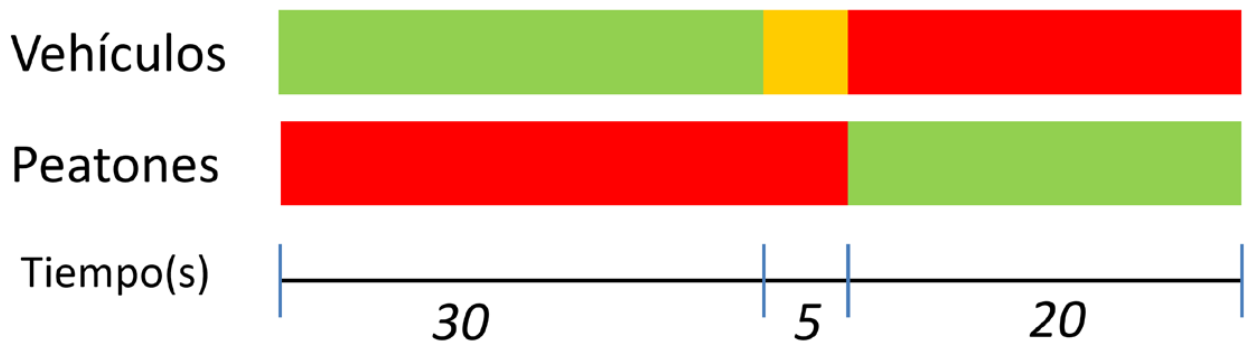
\includegraphics[width=8cm]{.images/CicloFuncionamiento.png}
\end{center}
Para ello, usaremos uno de los osciladores de cuarzo integrados en la propia
placa del laboratorio (DE2-115), que funciona a $50MHz$, y que mediante un
contador binario transformaremos en una señal de $4Hz$, es decir, un pulso cada
$0.25$ segundos.

El semáforo estará compuesto por cuatro luces LED, dos verdes y dos rojas. De
éstas, una de cada será para los peatones, y las otras dos para los coches, y
representaremos el color ámbar encendiendo a la vez los dos LED de vehículos.

\subsection*{Diseño del contador (\texttt{binary\_counter\_tc.v})}
Para el módulo del contador usaremos el dado en la práctica de laboratorio número
$5$, ya que mediante los parámetros podemos configurar el contador a nuestro
gusto. El código queda así:

\begin{lstlisting}[style={prettyverilog}]
module binary_counter_tc (CLK, CLK_ENA, RSTn, Q, LOADn, P , TC);
    parameter MODULE = 12500000; // Estos pueden ser valores arbitrarios, ya que los
    parameter WIDTH  = 24;       // modificamos despues.
    
    input CLK, CLK_ENA, RSTn, LOADn;
    input      [WIDTH-1:0] P;
    output                 TC;
    output reg [WIDTH-1:0] Q;

always @ (posedge CLK)
  begin
    if ( !RSTn )
      begin
        Q <= 0;
      end
    else if ( !LOADn)
        Q <= P;
    else if ( CLK_ENA)
        if ( Q == MODULE-1)
          begin
            Q <= 0;
          end
        else
          begin
            Q <= Q + 1;
          end
  end

    assign TC = (Q ==(MODULE-1))? CLK_ENA: 0;
endmodule
\end{lstlisting}

\end{document}
